\scanpage{105}

\mspage{111}

Le lemme implique qu'une \inserted{$\mathbb D=$}HOT-fibration \deleted{cohomologique} (au sens de la définition 2 page \deleted{\unsure{81}}\inserted{\unsure{101|103}} \deleted{\unsure{qui est de}} revue et corrigée à la page 96\unsure{,|-}97) est en fait déjà une HOT-fibration cohomologique et homologique complète. Or on a vu que si $f$ est \uline{propre}, $f$ est une $\unsure{\mathbb D|\mathrm{H}}$-fibration ssi les conditions équivalentes \uline{sur $Y$} (sans chgt. de base) sont satisfaites. Et dualement pour $f$ lisse :

\figure{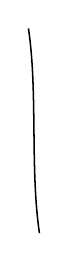
\begin{tikzpicture}[baseline]\draw[line width=.55pt] (0,2.6) .. controls (.12,1.8) and (.02,.8) .. (.14,0);\end{tikzpicture}}

\[
\searrow
\]

11.11.90

Je sens le besoin de réviser \deleted{\unsure{toutes}} les notions de $\mathbb D$-fibrations en tous genres \inserted{(p. \unsure{96|36} \unsure{ff|97})}. D'abord les diverses variantes utiles de l'axiome Der 3 sur les dérivateurs :

% slanted
\margin{Cf aussi la série \uline{Der} 3 c\unsure{\ldots} p. \unsure{114, 115|114--115}}

\uline{Der 3} a) si $Z\in\mathrm{Diag}$ est Hot-asphérique, il est $\mathbb D$-asphérique i.e. $\unsure{\mathcal A|A}=\mathbb D(e)\longrightarrow\mathbb D(Z)$ est pl. fidèle

a') Comme a), avec en plus la caractérisation de l'image essentielle de \deleted{\unsure{$\mathbb D$}} $\mathcal A$ dans $\mathbb D(Z)$, comme formée des $\mathbb D$-coeff. loc constants.

\uline{Der 3} b) Si $f:Z'\to Z$ de $\mathrm{Diag}$ est une Hot-équivalence, alors c'est une $\mathbb D$-équivalence, i.e. le foncteur $f^*:\mathbb D(Z)\to\mathbb D(Z')$ induit une \deleted{\unsure{fonction}}\inserted{équivalence} \deleted{pl. fidèle sur \unsure{la}} \inserted{entre les} sous-catégories formées des coefficients constants. (ou encore, un foncteur pl. fid $\mathbb D(Z)_{\mathrm{loc.const}}\longrightarrow\mathbb D(Z')$).

$b'_1)$ Si $f$ comme dessus, alors $f^{\unsure{\in|*}}$ est une $\mathbb D$-équivalence $1$-complète, i.e. le foncteur \deleted{\unsure{$f^*:\mathbb D(Z$}} $f^*:\mathbb D(Z)\to\mathbb D(Z')$ induit un foncteur pl fidèle

% archive sheet number: 105
